\chapter{Системийн Зохиомж}
\label{chapter4}

\section{Өгөгдлийн Ерөнхий Схем}
Өгөгдлийн ерөнхий схем нь системийн өгөгдлийн хоорондын харилцааг тодорхойлдог. Энэхүү системд дараах өгөгдлийн хүснэгтүүд ашиглагдана.

\subsection{Хэрэглэгч (User)}
\begin{itemize}
    \item \textbf{Primary Key (PK)}: UserID
    \item \textbf{Attributes}:
    \begin{itemize}
        \item UserName: Хэрэглэгчийн нэр
        \item Password: Нууц үг (hashed байдлаар хадгалах)
        \item Email: Имэйл хаяг
        \item RegistrationDate: Бүртгүүлсэн огноо
    \end{itemize}
\end{itemize}

\subsection{Хувцас (Clothes)}
\begin{itemize}
    \item \textbf{Primary Key (PK)}: ClothesID
    \item \textbf{Attributes}:
    \begin{itemize}
        \item Name: Хувцасны нэр
        \item Type: Хувцасны төрөл (хүрэм, цамц гэх мэт)
        \item Size: Хэмжээ (S, M, L гэх мэт)
        \item Color: Өнгө
        \item Material: Материал (даавуу, арьс гэх мэт)
        \item Price: Үнэ
    \end{itemize}
\end{itemize}

\subsection{Шүүгээ (Wardrobe)}
\begin{itemize}
    \item \textbf{Primary Key (PK)}: WardrobeID
    \item \textbf{Foreign Key (FK)}: UserID
    \item \textbf{Attributes}:
    \begin{itemize}
        \item ClothesID: Хувцасны ID
        \item AddedDate: Шүүгээнд нэмэгдсэн огноо
    \end{itemize}
\end{itemize}

\subsection{Санал Болгох Түүх (RecommendationHistory)}
\begin{itemize}
    \item \textbf{Primary Key (PK)}: RecommendationID
    \item \textbf{Foreign Key (FK)}: UserID
    \item \textbf{Attributes}:
    \begin{itemize}
        \item ClothesID: Санал болгосон хувцасны ID
        \item Date: Санал болгосон огноо
    \end{itemize}
\end{itemize}

\section{Зохиомжийн Шатны Класс Диаграм}
Класс диаграм нь системийн объектуудын хоорондын харилцааг тодорхойлдог. 

\begin{figure}[h!]
    \centering
    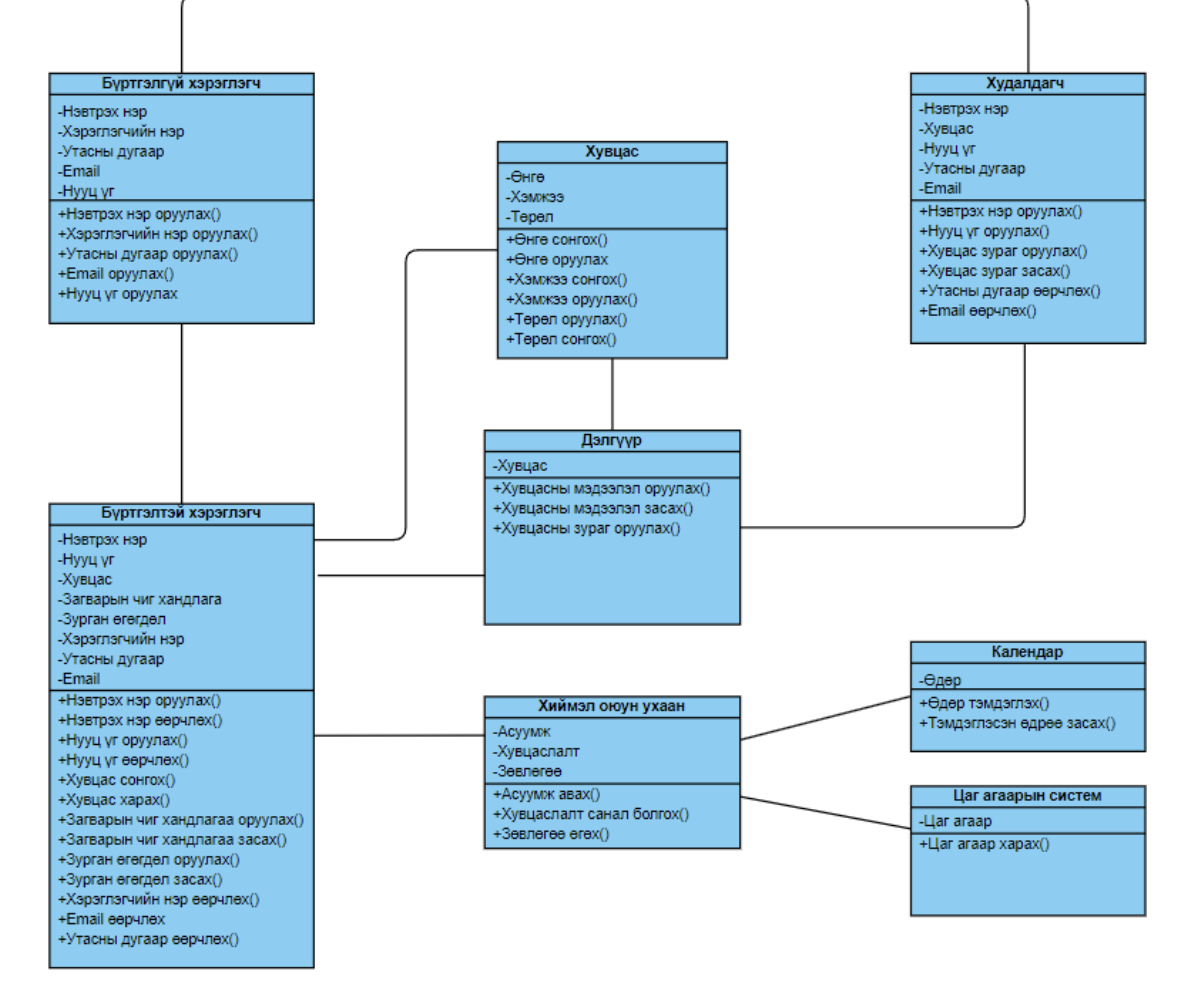
\includegraphics[width=0.8\textwidth]{figures/Screenshot 2024-12-12 at 17.15.40.png}
    \caption{Класс диаграмын жишээ}
    \label{fig:class-diagram}
\end{figure}
\section{Зохиомжийн Шатны Дарааллын Диаграм}

Энэхүү диаграм нь хэрэглэгчийн хувцас хайх, санал болгох, худалдан авах үйлдлүүдийн дарааллыг харуулж байна. Хэрэглэгч хувцас хайж, санал болгосон хувцаснуудаас сонголт хийж, худалдан авах үйлдлийг системд дамжуулж байна.

\begin{figure}[h!]
    \centering
    \begin{tikzpicture}[node distance=4cm, auto]
        % Actors and Objects
        \node[rectangle, draw] (user) {Хэрэглэгч};
        \node[rectangle, draw, right of=user, xshift=3cm] (system) {Систем};
        \node[rectangle, draw, right of=system, xshift=3cm] (clothes) {Хувцаснууд};
        \node[rectangle, draw, below of=clothes] (weather) {Цаг Агаар};
        
        % Messages
        \draw[->] (user) -- node[midway, above] {Хувцас хайх} (system);
        \draw[->] (system) -- node[midway, above] {Хэрэглэгчийн сонголт авах} (clothes);
        \draw[->] (system) -- node[midway, above] {Цаг агаарын мэдээлэл авах} (weather);
        \draw[->] (weather) -- node[midway, right] {Цаг агаарын мэдээлэл} (system);
        \draw[->] (clothes) -- node[midway, below] {Санал болгосон хувцас} (system);
        \draw[->] (system) -- node[midway, below] {Хувцас санал болгох} (user);
        
    \end{tikzpicture}
    \caption{Зохиомжийн Шатны Дарааллын Диаграм: Хувцас Санал Болгох}
    \label{fig:sequence-diagram}
\end{figure}


\section{Төлөвийн Диаграм}
Төлөвийн диаграм нь системийн объектуудын төлөвүүд болон тэдгээрийн шилжилтийг тодорхойлно.

\begin{figure}[h!]
    \centering
    \begin{tikzpicture}[->, node distance=2cm, auto]
        % Nodes
        \node[circle, draw] (idle) {Idle};
        \node[circle, draw, below of=idle] (search) {Хувцас Хайх};
        \node[circle, draw, right of=search, xshift=2cm] (recommend) {Санал Болгох};
        \node[circle, draw, below of=search] (add) {Хувцас Нэмэх};
        \node[circle, draw, below of=add] (logout) {Гарах};
        
        % Arrows
        \draw[->] (idle) -- node[midway, right] {Хэрэглэгч орж ирэх} (search);
        \draw[->] (search) -- node[midway, above] {Санал гаргах} (recommend);
        \draw[->] (search) -- node[midway, left] {Шүүгээнд нэмэх} (add);
        \draw[->] (add) -- node[midway, left] {Үйлдлийг дуусгах} (logout);
    \end{tikzpicture}
    \caption{Системийн төлөвийн диаграм}
    \label{fig:state-diagram}
\end{figure}

\section{Дэлгэцийн Зохиомж}
Системийн дэлгэцүүд нь энгийн, хэрэглэгчдэд ойлгомжтой байх шаардлагатай. 

\subsection{Нүүр Хуудас}
\begin{itemize}
    \item Хувийн шүүгээний жагсаалт
    \item Өнөөдрийн цаг агаарын мэдээлэл
    \item Санал болгосон хослолын зураг, мэдээлэл
\end{itemize}

\begin{figure}[h!]
    \centering
    \includegraphics[width=0.7\textwidth]{figures/Screenshot 2024-12-12 at 17.26.39.png}
    \caption{Нүүр хуудасны загвар}
    \label{fig:homepage-design}
\end{figure}

\subsection{Хувцас Нэмэх}
Хувцасны төрөл, өнгө, материал зэрэг талбаруудтай.

\section{Тайлан, Статистик Үзүүлэлтийн Загвар}

Энэхүү хэсэгт хувцасны ашиглалтын статистик, цаг агаарын өгөгдөлтэй холбогдсон санал болгох үйлдлүүдийн үр дүнг гарган, хэрэглэгчдэд хамгийн тохиромжтой хувцас санал болгох үйл ажиллагааг тодорхойлохоор төлөвлөж байна. Систем нь хэрэглэгчдийн хувцасны хандлага, хэрэглээ, агаарын төлөв байдлыг харгалзан, хувцаснуудын зохимжтой байдлыг хэрхэн сайжруулах талаар тусламж үзүүлнэ.

\subsection{Хувцасны Ашиглалтын Статистик}
Хэрэглэгчдийн хувцасны ашиглалт, сонголт, өөрчлөлтүүдийн тухай өгөгдөл хураагдаж, тухайн хувцаснуудын эрэлт хэрэгцээ болон ашиглалтын давтамжийг тогтооно. Жишээлбэл:
\begin{itemize}
    \item \textbf{Хувцасны төрлүүдийн хэрэглээ:} Өдөр тутмын хувцас, спорт хувцас, албан хувцас гэх мэт.
    \item \textbf{Хэрэглэгчийн нас, хүйсийн онцлог:} Эрэгтэй, эмэгтэй хэрэглэгчдийн хувцасны сонголт.
    \item \textbf{Хувцасны үр дүнтэй хугацаа:} Хувцаснуудын ашиглалтын хугацаа, жишээлбэл, аль хувцас нь хамгийн олон удаа сонгогддог.
\end{itemize}

\subsection{Цаг Агаарын Үзүүлэлтүүдтэй Холбогдсон Санал Болгох}
Цаг агаарын өөрчлөлт, улирлын онцлогт тохирсон хувцасны сонголтуудыг санал болгох нь хэрэглэгчдэд хамгийн тохиромжтой хувцас сонгох нөхцөлийг бүрдүүлнэ. Энэ хэсэгт цаг агаарын температур, салхи, хур тунадас гэх мэт үзүүлэлтүүдийг харгалзан хувцасны санал болон үнийн саналуудыг гаргах аргачлал танилцуулах болно.

\section{Бүлгийн Дүгнэлт}

Энэхүү бүлэгт бид системийн бүх хэсгүүдийг нэгтгэн дүгнэх бөгөөд түүний үр дүнгүүдийг өргөн хүрээнд хэлэлцэнэ. Систем нь хэрэглэгчдийн хэрэгцээ, хүсэлтийн дагуу хувцас санал болгох, цаг агаарын нөхцөлд тохирсон хувцасны сонголт хийх зэргээр хэрэглэгчдэд амар хялбар, тухтай үйлчилгээг үзүүлэхийг зорьж байна.

\subsection{Ерөнхий Дүгнэлт}
Систем нь хэрэглэгчдийн хувцасны сонголтыг сайжруулах, агаарын нөхцөл болон улирлын онцлогт үндэслэн хувцас санал болгох, хэрэглэгчийн сэтгэл ханамжийг дээшлүүлэх зорилгоор бүтээсэн. Хэрэглэгчдийн өгөгдлийг хураан, цаг агаарын мэдээллийг ашиглан, хувцасны хамгийн тохиромжтой сонголтыг санал болгох боломжийг бий болгоно. Энэ нь хэрэглэгчдийн хувцасны эрэлт, хэрэгцээг амжилттай хангаснаар платформын үр ашигтай байдалд эерэг нөлөө үзүүлэх болно.

\subsection{Хэрэглэгчдэд Зориулсан Найдвартай Платформ}
Систем нь хэрэглэгчдэд хэрэглэж болох хамгийн сайн платформыг бий болгоход чиглэгдсэн бөгөөд энэ нь өндөр чанартай өгөгдөл, цаг агаарын мэдээллийг үндэслэн хувцасны зөвлөгөө өгөх, хувцас худалдах, түрээслэх зэрэг үйлдлүүдийг аюулгүй, найдвартай гүйцэтгэх боломжтой. Платформ нь хэрэглэгчийн хэрэгцээг хамгийн өндөр хэмжээгээр хангах, хамгийн сайн үйлчилгээ үзүүлэх үүднээс тасралтгүй сайжруулалт хийж байгаа.

\subsection{Төслийн Ирээдүйн Чиг Хандлага}
Цаашид, энэхүү системийг илүү өргөн хүрээнд хөгжүүлж, хэрэглэгчдэд хамгийн тохиромжтой хувцасны санал, сонголтыг цаг агаар, улирлын өөрчлөлтүүдтэй тохирч гаргах боломжийг бүрдүүлэх шаардлагатай. Мөн, хэрэглэгчийн өгөгдлийг илүү олон төрлийн параметрүүдээр нэмэгдүүлж, зөвхөн хувцасны сонголт төдийгүй хэрэглэгчийн бусад шаардлагыг ч хангах өргөн боломжийг хөгжүүлэх шаардлагатай.


\section{Ерөнхий Дүгнэлт}

Энэхүү систем нь хэрэглэгчийн хувцасны сонголт, цаг агаарын нөхцөлд тохирсон хувцас санал болгох шийдлийг санал болгож байна. Хэрэглэгчийн хандлагыг, хувцасны эрэлт хэрэгцээг тооцоолох замаар хамгийн тохиромжтой хувцасны санал гаргахад анхаарсан бөгөөд энэ нь хэрэглэгчийн сэтгэл ханамжийг дээшлүүлэх, хувцасны сонголтыг хөнгөвчлөх зорилготой.

\subsection{Системийн Гол Чиг Хандлага}
Систем нь хоёр үндсэн чиглэлээр үйл ажиллагаагаа явуулдаг. Нэгдүгээрт, систем нь хэрэглэгчийн өгөгдлийг ашиглан, хэрэглэгчийн сонирхол, хувцасны хэрэглээний хэв маягийг шинжилж, хамгийн тохиромжтой хувцас санал болгоход чиглэгдэнэ. Хоёрдугаарт, систем нь цаг агаарын өгөгдлийг ашиглан, улирлын болон цаг агаарын өөрчлөлтөд тохирсон хувцасны сонголтыг хийж, хэрэглэгчдэд цаг агаарын нөхцөлд нийцсэн хувцас санал болгох боломжийг бүрдүүлнэ.

\subsection{Хэрэглэгчдэд Тохиромжтой Үйлчилгээ}
Систем нь хэрэглэгчдэд хамгийн тохиромжтой хувцасны сонголтыг санал болгохоор төлөвлөгдсөн бөгөөд агаарын төлөв байдлыг үндэслэн хувцас санал болгох үйлдлүүдийг автоматжуулсан. Өдөр тутмын хувцас, спорт хувцас, албан хувцас гэх мэт төрөл бүрийн хувцаснуудын дунд хэрэглэгчийн шаардлагад нийцсэн хувцас сонголтыг зөвшөөрнө. Мөн систем нь хэрэглэгчдийн өнгөрсөн ашиглалтын мэдээллийг авч, хувцасны хандлагыг сайтар ойлгож, цаашдын санал болгох үйл ажиллагааг илүү тохиромжтой болгоно.

\subsection{Цаг Агаарын Нөхцөлд Тохирсон Санал Болгох}
Цаг агаарын нөхцөл нь хувцасны сонголтод хамгийн их нөлөөлдөг хүчин зүйлүүдийн нэг бөгөөд энэ систем нь цаг агаарын мэдээллийг авч, хэрэглэгчдэд тохирсон хувцас санал болгохоор зорилт тавьсан. Систем нь температур, салхи, хур тунадас зэргийн мэдээллийг ашиглан, өдөр тутмын хувцас, аялалын хувцас зэрэг сонголтуудыг цаг агаарын нөхцөлд тулгуурлан гаргах болно.

\subsection{Системийн Амжилттай Хэрэглээ}
Систем нь хэрэглэгчдийн хэрэгцээг хангах, хувцасны сонголтыг хялбаршуулах, мөн хамгийн тохиромжтой хувцас санал болгох боломжийг олгодог. Хэрэглэгчийн хувцасны сонголт, хүсэлтийг анализ хийж, энэ мэдээллийг цаг агаар болон улирлын онцлогтой хослуулан хэрэглэгчийн хүссэн хувцасыг зөв санал болгох нь системийн гол давуу тал юм.

\subsection{Цаашдын Хөгжил, Сайжруулалт}
Цаашид энэхүү системийг илүү өргөн хүрээнд хөгжүүлж, хэрэглэгчийн нэмэлт өгөгдлийг хүлээн авах, хувцасны загвар болон хандлагыг илүү нарийвчлалтай шинжлэх боломжийг нэмэгдүүлэх шаардлагатай. Мөн, хэрэглэгчийн сэтгэл ханамжийн дүн шинжилгээ, хувцасны эрэлт хэрэгцээг бүрэн гүйцэд тооцоолох хэрэгцээтэй байгаа бөгөөд энэ нь ирээдүйд системийг илүү ухаалаг, нээлттэй платформ болгоход нөлөөлнө.

\chapter*{Ашигласан Материал}
\begin{enumerate}
    \item Internet Live Stats. \textit{Internet Users Statistics}. \url{http://www.internetlivestats.com/internet-users}
    \item David Smith. \textit{iOS Version Stats}. \url{https://david-smith.org/iosversionstats/}
\end{enumerate}
\end{document}